\section{Estructura Organizacional} \label{sect:Estructura_organizacional}

Empresas TD es una compañía con una gran proyección a futuro compuesta mayormente 
por gente joven. El perfil buscado en los miembros del equipo de trabajo es el de 
un profesional dinámico, creativo e innovador, comprometido por brindar a los
asociados y usuarios experiencias de alta calidad. 

Actualmente se gestionan 4 proyectos en Empresas TD, como se puede ver en la figura \ref{fig:ogtd}y se describen a continuación:

\begin{figure}[h]
	\begin{center}
		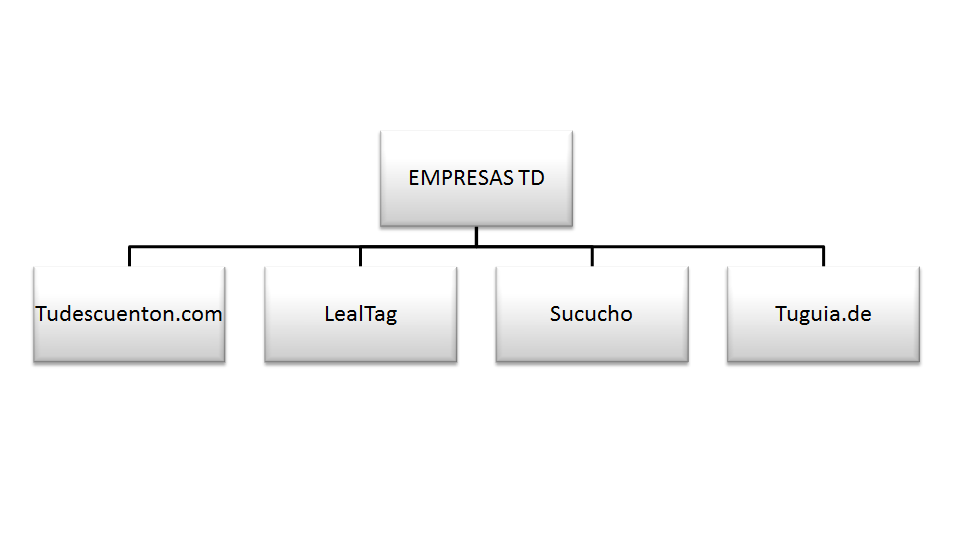
\includegraphics[scale=0.4]{imagenes/OrganigramaTD.png}
	\end{center}
	\caption{
		\label{fig:ogtd}
		Organigrama de Empresas TD.
	}
\end{figure}



\begin{itemize}
  \item \textbf{Tudescuenton:} es el sistema que le brinda a los venezolanos, la oportunidad de conocer las mejores cosas que hacer, en las principales ciudades del país, a través de descuentos insuperables\cite{TDC}.
  \item \textbf{Lealtag:} LealTag es la plataforma que te permite recibir premios, descuentos y regalos en tus sitios favoritos por ser un cliente frecuente\cite{LTG}.
  \item \textbf{Sucucho:} es un portal que ofrece a los creativos venezolanos un espacio en donde pueden exponer su talento ante el país, en el cual brindamos la oportunidad de que cada uno tenga su tiendita propia 365 días al año\cite{SCC}.
  \item \textbf{Tuguiade:} Tuguía.de es una página que sirve para conectar los locales con sus clientes. Ofreciéndoles a los usuarios información verificada de los mismos y la posibilidad de escribir sobre sus experiencias, subir fotos e intercambiar historias con los otros clientes\cite{TGD}. 
\end{itemize}
  
Cada proyecto tiene asignado un director general y un esquema organizacional específico que se ajusta a sus necesidades. En el caso de Tuguia.de; proyecto en el que desarrolló el proyecto de pasantía, el organigrama se muestra en la figura \ref{fig:ogtgd}donde se puede observar la estructura organizativa de la que el pasante fue parte. 

\begin{figure}[h]
	\begin{center}
		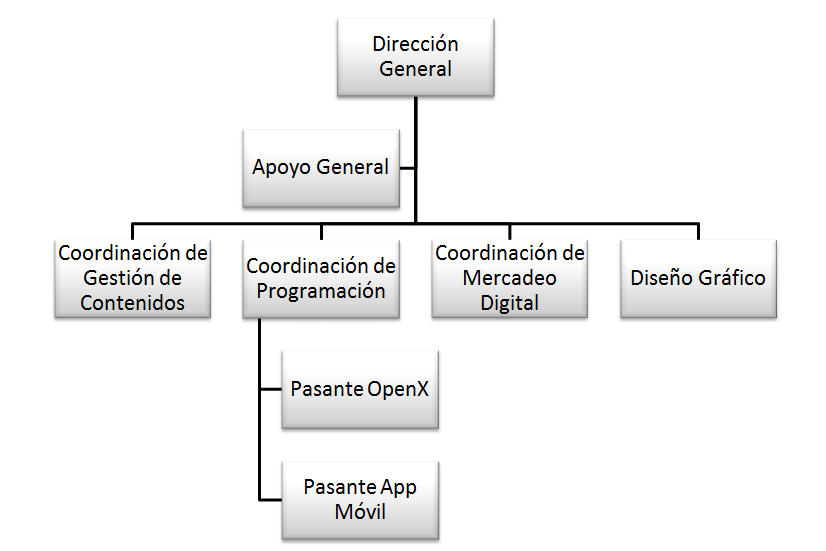
\includegraphics[scale=0.4]{imagenes/OrganigramaTGD.png}
	\end{center}
	\caption{
		\label{fig:ogtgd}
		Organigrama de Tuguia.de
	}
\end{figure}
 